\documentclass[10pt]{standalone}
\usepackage{tikz}
\usepackage{chemfig}
\usepackage[UTF8]{ctex}
\usepackage[version=4]{mhchem}
\usetikzlibrary{intersections,calc,backgrounds,knots}
\standaloneconfig{border=0.0}
\begin{document}

$
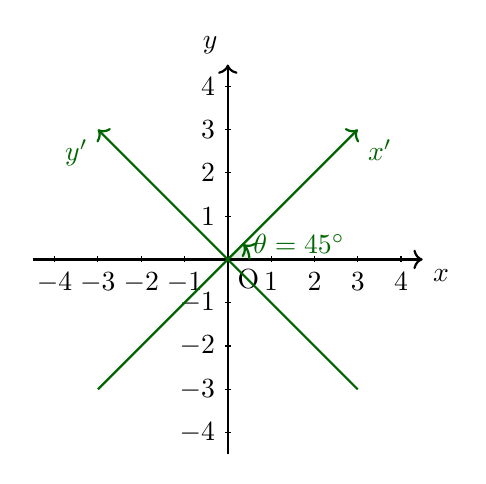
\begin{tikzpicture}[scale=0.55] \definecolor{color1bg}{HTML}{006400} \filldraw[fill=color1bg!10] (0.5,0) arc(0:45:0.5) -- (0,0); \node[anchor=north west](0,0) {O}; \filldraw[fill=black] (0,0) circle(0.05); \draw[thick, ->] (-4.5,0) -- (4.5,0) node[anchor=north west] {$x$}; \draw[thick, ->] (0,-4.5) -- (0,4.5) node[anchor=south east] {$y$}; \foreach \x in{-4,-3,-2,-1,1,2,3,4} \draw (\x cm,2pt) -- (\x cm,-2pt) node[anchor=north] {$\x$}; \foreach \y in{-4,-3,-2,-1,1,2,3,4} \draw (2pt,\y cm) -- (-2pt,\y cm) node[anchor=east] {$\y$}; \draw[thick, ->,color1bg] (-3,-3) -- (3,3) node[anchor=north west] {$x'$}; \draw[thick, ->,color1bg] (3,-3) -- (-3,3) node[anchor=north east] {$y'$}; \draw[thick,->,color1bg] (0.5,0) arc(0:45:0.5) node[anchor=west] {$\theta = 45^\circ$}; \end{tikzpicture}
$

\end{document}